% ============================================================
% TERM PROJECT – PROPOSAL
% Databases · THGA Bochum
% ============================================================

\documentclass[11pt,a4paper]{article}

\usepackage{thga-db}
\usepackage{caption}
\usepackage{tikz}
\usetikzlibrary{positioning,arrows.meta,shapes.multipart}

\renewcommand{\thgaKurs}{Databases}
\renewcommand{\thgaDatum}{Summer Term 2026}
\newcommand{\authorName}{Meriem Mornagui}
\newcommand{\projectTitle}{Vulnerability Tracking System}

\begin{document}

\thispagestyle{empty}
\thgaTitel{Term Project -- Proposal}{\projectTitle}

\begin{infobox}
\textbf{Author:} \authorName \\
\textbf{Module:} Introduction to Database Management Systems · THGA Bochum \\
\textbf{Submitted to:} Stephan Bökelmann · \href{mailto:sboekelmann@ep1.rub.de}{sboekelmann@ep1.rub.de} \\
\textbf{Planned effort:} approximately 40 hours over no more than two months
\end{infobox}

% ============================================================
\section{Application domain and motivation}
% ============================================================

Large organisations manage many IT assets across on-premises and cloud
environments. They must know which assets are affected by known vulnerabilities
(CVEs), which team owns each asset, who is responsible for remediation, and
whether remediation deadlines are being met. Spreadsheets quickly become
difficult to maintain because they cannot reliably enforce relationships,
validate status values, prevent duplicate findings, or answer analytical
questions without manual work.

The proposed application replaces this spreadsheet-based process with a
relational database, a REST API, and a desktop frontend. It manages teams, IT
assets, known vulnerabilities, and findings that connect affected assets to
vulnerabilities. Each finding records its status, discovery date, remediation
deadline, and optional resolution date.

The project is inspired by real-world vulnerability-management workflows, but
it is an independent educational prototype. Only fictional teams, assets,
addresses, vulnerabilities, dates, and credentials will be used. No internal
company data, code, screenshots, or documentation will be included.

\textbf{Usage scenario 1.} A security analyst opens the frontend and filters the
findings for severity \emph{Critical} and status \emph{Open}. The analyst sees
the affected asset and its responsible team and can create or resolve findings
through the API.

\textbf{Usage scenario 2.} A team lead requests all overdue findings belonging
to their team. The system returns the affected assets, CVE identifiers,
severity levels, and past-due remediation dates so that the team can prioritise
its work.

% ============================================================
\section{Data model -- ER diagram}
% ============================================================

Figure~\ref{fig:er} shows four entity types. A team owns one or more assets. An
asset represents a physical or virtual IT resource such as a server, laptop, or
cloud instance. A vulnerability represents a known security weakness identified
by a unique CVE identifier and a severity level. A finding links one asset to
one vulnerability and stores remediation-specific information.

One asset may be affected by many vulnerabilities, and one vulnerability may
affect many assets. Therefore, asset and vulnerability have an N:M relationship.
The associative entity \texttt{finding} resolves this relationship into two
1:N relationships.

\begin{figure}[ht]
\centering
\begin{tikzpicture}[
  entity/.style={draw=THGABlau!70, fill=THGABlau!5, rounded corners=2pt,
                 minimum width=4.2cm, align=left, font=\small},
  rel/.style={-Latex, thick, draw=THGABlau!75},
  node distance=1.6cm and 2.3cm
]

\node[entity] (team) {
  \textbf{TEAM}\\[-1mm]
  \underline{id}\\
  name\\
  contact\_email
};

\node[entity, right=of team] (asset) {
  \textbf{ASSET}\\[-1mm]
  \underline{id}\\
  name\\
  type\\
  \emph{team\_id}
};

\node[entity, below=of asset] (finding) {
  \textbf{FINDING}\\[-1mm]
  \underline{id}\\
  \emph{asset\_id}\\
  \emph{vulnerability\_id}\\
  status\\
  discovered\_on\\
  due\_date\\
  resolved\_on
};

\node[entity, left=of finding] (vuln) {
  \textbf{VULNERABILITY}\\[-1mm]
  \underline{id}\\
  cve\_id\\
  severity\\
  description
};

\draw[rel] (team) -- node[above,font=\small]{\(1\) owns \(N\)} (asset);
\draw[rel] (asset) -- node[right,font=\small]{\(1\) has \(N\)} (finding);
\draw[rel] (vuln) -- node[below,font=\small]{\(1\) appears in \(N\)} (finding);

\end{tikzpicture}
\caption{ER diagram of the Vulnerability Tracking System, including entities,
key attributes, foreign keys, relationships, and cardinalities. The N:M
relationship between \texttt{asset} and \texttt{vulnerability} is resolved by
\texttt{finding}.}
\label{fig:er}
\end{figure}

% ============================================================
\section{From model to relational schema}
% ============================================================

The relational schema is derived directly from the ER diagram. Primary keys are
underlined and foreign keys are written in italics.

\begin{itemize}
  \item \texttt{team}(\underline{id}, name, contact\_email)
  \item \texttt{asset}(\underline{id}, name, type, \emph{team\_id})
  \item \texttt{vulnerability}(\underline{id}, cve\_id, severity, description)
  \item \texttt{finding}(\underline{id}, \emph{asset\_id},
        \emph{vulnerability\_id}, status, discovered\_on, due\_date,
        resolved\_on)
\end{itemize}

The database uses the following integrity constraints:

\begin{itemize}
  \item \texttt{team.name} and \texttt{vulnerability.cve\_id} are unique.
  \item The combination \texttt{(asset\_id, vulnerability\_id)} is unique, so
        the same vulnerability cannot be added twice to the same asset.
  \item \texttt{severity} is restricted to \emph{Critical}, \emph{High},
        \emph{Medium}, or \emph{Low} by a \texttt{CHECK} constraint.
  \item \texttt{status} is restricted to \emph{Open}, \emph{In Progress}, or
        \emph{Resolved} by a \texttt{CHECK} constraint.
  \item \texttt{due\_date} must not be earlier than \texttt{discovered\_on}.
  \item \texttt{resolved\_on} must be present only when the status is
        \emph{Resolved}.
\end{itemize}

\textbf{Normalisation.} The schema is in third normal form (3NF). Each table
represents one subject, every non-key attribute depends on its table's primary
key, and no non-key attribute depends transitively on another non-key attribute.
Team information is stored once in \texttt{team}; asset records reference it
through \texttt{team\_id}. Vulnerability descriptions and severity levels are
stored once in \texttt{vulnerability}, while \texttt{finding} stores only
relationship-specific remediation data.

% ============================================================
\section{API design}
% ============================================================

The REST API is implemented with FastAPI. Read operations do not require an API
key. Write operations require a valid \texttt{X-API-Key} header. Request bodies
and responses are validated with Pydantic models, while SQL queries use
parameters rather than string concatenation.

\renewcommand{\arraystretch}{1.2}
\begin{tabularx}{\linewidth}{@{}p{1.6cm}p{4.2cm}X@{}}
\toprule
\textbf{Method} & \textbf{Path} & \textbf{Purpose} \\
\midrule
\texttt{GET} & \texttt{/assets} & List assets with team name and number of open
findings (JOIN + aggregation). \\
\texttt{GET} & \texttt{/findings} & List findings with asset, team, CVE,
severity, status, and dates (multiple JOINs); optional filters. \\
\texttt{GET} & \texttt{/findings/\{id\}} & Return the complete details of one
finding. \\
\texttt{POST} & \texttt{/findings} & Create a finding after validating foreign
keys and duplicate combinations; requires \texttt{X-API-Key}. \\
\texttt{POST} & \texttt{/findings/\{id\}/resolve} & Change an open finding to
\emph{Resolved} and set the resolution date; requires \texttt{X-API-Key}. \\
\bottomrule
\end{tabularx}

For example,
\texttt{GET /findings?status=Open\&severity=Critical} returns only open critical
findings. The endpoint \texttt{GET /assets} joins \texttt{asset} and
\texttt{team}, left-joins \texttt{finding}, and groups the result by asset to
calculate the number of open findings.

% ============================================================
\section{Frontend prototype}
% ============================================================

The frontend is a Python/tkinter desktop application. It communicates only with
the REST API and never connects directly to PostgreSQL. At startup, an initial
connection dialog requests the API URL and API key. The key is kept in memory
for the current session and is not written to disk. The main window provides an
asset overview and access to the finding list, creation form, and resolution
action.

Figures~\ref{fig:fe-connect}--\ref{fig:fe-resolve} show the planned user
interface. Figure~\ref{fig:fe-connect} collects the connection information.
Figure~\ref{fig:fe-main} displays the asset overview and aggregated number of
open findings. Figure~\ref{fig:fe-create} provides the validated input fields
needed to create a finding. Figure~\ref{fig:fe-resolve} shows the confirmation
step used to resolve an existing finding.

\begin{figure}[ht]
\centering
\begin{minipage}[t]{0.47\linewidth}\centering
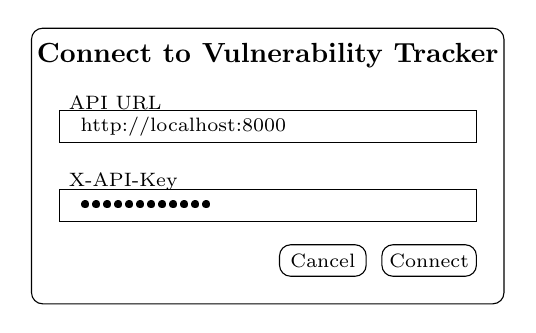
\begin{tikzpicture}[font=\scriptsize]
  \draw[rounded corners] (0,0) rectangle (6,3.5);
  \node[font=\bfseries] at (3,3.15) {Connect to Vulnerability Tracker};
  \node[anchor=west] at (0.35,2.55) {API URL};
  \draw (0.35,2.05) rectangle (5.65,2.45);
  \node[anchor=west] at (0.5,2.25) {http://localhost:8000};
  \node[anchor=west] at (0.35,1.55) {X-API-Key};
  \draw (0.35,1.05) rectangle (5.65,1.45);
  \node[anchor=west] at (0.5,1.25) {••••••••••••};
  \draw[rounded corners] (3.15,0.35) rectangle (4.25,0.75);
  \draw[rounded corners] (4.45,0.35) rectangle (5.65,0.75);
  \node at (3.7,0.55) {Cancel};
  \node at (5.05,0.55) {Connect};
\end{tikzpicture}
\captionof{figure}{Initial connection dialog for the API URL and
\texttt{X-API-Key}.}
\label{fig:fe-connect}
\end{minipage}\hfill
\begin{minipage}[t]{0.47\linewidth}\centering
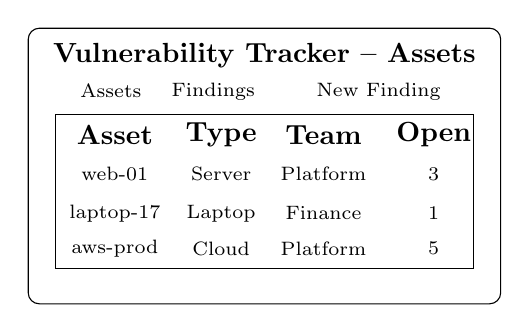
\begin{tikzpicture}[font=\scriptsize]
  \draw[rounded corners] (0,0) rectangle (6,3.5);
  \node[font=\bfseries] at (3,3.15) {Vulnerability Tracker -- Assets};
  \node at (1.05,2.7) {Assets};
  \node at (2.35,2.7) {Findings};
  \node at (4.45,2.7) {New Finding};
  \draw (0.35,0.45) rectangle (5.65,2.4);
  \node[font=\bfseries] at (1.1,2.15) {Asset};
  \node[font=\bfseries] at (2.45,2.15) {Type};
  \node[font=\bfseries] at (3.75,2.15) {Team};
  \node[font=\bfseries] at (5.15,2.15) {Open};
  \node at (1.1,1.65) {web-01}; \node at (2.45,1.65) {Server};
  \node at (3.75,1.65) {Platform}; \node at (5.15,1.65) {3};
  \node at (1.1,1.15) {laptop-17}; \node at (2.45,1.15) {Laptop};
  \node at (3.75,1.15) {Finance}; \node at (5.15,1.15) {1};
  \node at (1.1,0.7) {aws-prod}; \node at (2.45,0.7) {Cloud};
  \node at (3.75,0.7) {Platform}; \node at (5.15,0.7) {5};
\end{tikzpicture}
\captionof{figure}{Main asset screen populated by \texttt{GET /assets}.}
\label{fig:fe-main}
\end{minipage}

\vspace{1em}

\begin{minipage}[t]{0.47\linewidth}\centering
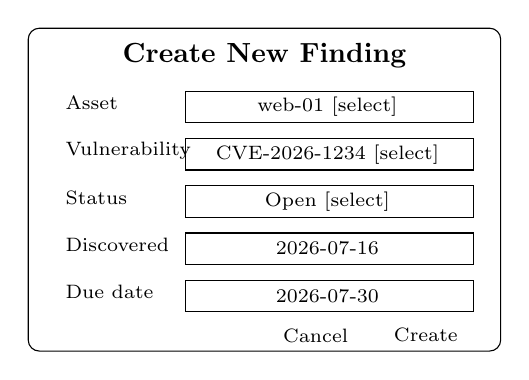
\begin{tikzpicture}[font=\scriptsize]
  \draw[rounded corners] (0,0) rectangle (6,4.1);
  \node[font=\bfseries] at (3,3.75) {Create New Finding};
  \node[anchor=west] at (0.35,3.15) {Asset};
  \draw (2.0,2.9) rectangle (5.65,3.3); \node at (3.8,3.1) {web-01 [select]};
  \node[anchor=west] at (0.35,2.55) {Vulnerability};
  \draw (2.0,2.3) rectangle (5.65,2.7); \node at (3.8,2.5) {CVE-2026-1234 [select]};
  \node[anchor=west] at (0.35,1.95) {Status};
  \draw (2.0,1.7) rectangle (5.65,2.1); \node at (3.8,1.9) {Open [select]};
  \node[anchor=west] at (0.35,1.35) {Discovered};
  \draw (2.0,1.1) rectangle (5.65,1.5); \node at (3.8,1.3) {2026-07-16};
  \node[anchor=west] at (0.35,0.75) {Due date};
  \draw (2.0,0.5) rectangle (5.65,0.9); \node at (3.8,0.7) {2026-07-30};
  \node at (3.65,0.2) {Cancel}; \node at (5.05,0.2) {Create};
\end{tikzpicture}
\captionof{figure}{Finding creation form using \texttt{POST /findings}.}
\label{fig:fe-create}
\end{minipage}\hfill
\begin{minipage}[t]{0.47\linewidth}\centering
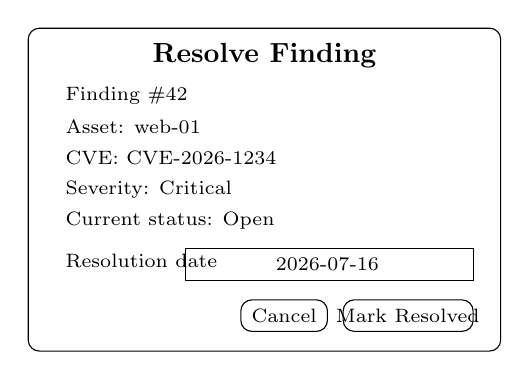
\begin{tikzpicture}[font=\scriptsize]
  \draw[rounded corners] (0,0) rectangle (6,4.1);
  \node[font=\bfseries] at (3,3.75) {Resolve Finding};
  \node[anchor=west] at (0.35,3.25) {Finding \#42};
  \node[anchor=west] at (0.35,2.85) {Asset: web-01};
  \node[anchor=west] at (0.35,2.45) {CVE: CVE-2026-1234};
  \node[anchor=west] at (0.35,2.05) {Severity: Critical};
  \node[anchor=west] at (0.35,1.65) {Current status: Open};
  \node[anchor=west] at (0.35,1.15) {Resolution date};
  \draw (2.0,0.9) rectangle (5.65,1.3); \node at (3.8,1.1) {2026-07-16};
  \draw[rounded corners] (2.7,0.25) rectangle (3.8,0.65);
  \draw[rounded corners] (4.0,0.25) rectangle (5.65,0.65);
  \node at (3.25,0.45) {Cancel};
  \node at (4.82,0.45) {Mark Resolved};
\end{tikzpicture}
\captionof{figure}{Resolution screen using
\texttt{POST /findings/\{id\}/resolve}.}
\label{fig:fe-resolve}
\end{minipage}
\end{figure}

The application will be packaged as a Debian \texttt{.deb} installer. The Python
application will first be bundled with PyInstaller and then packaged with
\texttt{fpm}.

% ============================================================
\section{Operation with Docker Compose}
% ============================================================

The backend consists of two Docker containers orchestrated with Docker Compose.
The \texttt{postgres} service creates the schema and seed data from an
\texttt{init.sql} script on first startup. The \texttt{api} service is built
from the \texttt{api/} directory, waits for a healthy database connection, and
exposes FastAPI on port 8000.

Database credentials and the API key are read from a \texttt{.env} file that is
excluded from Git. The repository contains a \texttt{.env.example} file with
safe placeholder values so that the required variables are documented without
publishing secrets.

Deployment on the lecture server consists of the following steps:

\begin{enumerate}
  \item Copy \texttt{.env.example} to \texttt{.env} and set secure values.
  \item Run \texttt{docker compose up -d --build} to start PostgreSQL and the API.
  \item Verify the services with \texttt{docker compose ps} and the API health
        endpoint.
  \item Install the frontend with
        \texttt{sudo dpkg -i vuln-tracker\_0.1.0\_amd64.deb}.
  \item Launch \texttt{vuln-tracker} and enter the API URL and API key.
\end{enumerate}

% ============================================================
\section{Scope, milestones and risks}
% ============================================================

\textbf{Scope.} The minimum viable product contains four tables, five REST
endpoints, one tkinter desktop application with four principal screens, Docker
Compose deployment, automated tests, documentation, and a short demonstration
video. User accounts, external CVE feeds, e-mail notifications, and historical
status auditing are explicitly outside the project scope.

\textbf{Milestones and schedule.}

\renewcommand{\arraystretch}{1.2}
\begin{tabularx}{\linewidth}{@{}p{1.4cm}Xp{1.8cm}@{}}
\toprule
\textbf{Week} & \textbf{Milestone} & \textbf{Est. hours} \\
\midrule
1 & Final ER model, SQL schema, constraints, seed data, and local Docker Compose
setup & 8 \\
2--3 & FastAPI models and all endpoints, authentication guard, JOIN and
aggregation queries & 12 \\
4--5 & tkinter frontend, API integration, validation, and Debian packaging & 12 \\
6 & Automated tests, deployment verification, documentation, and video & 8 \\
\bottomrule
\end{tabularx}

\textbf{Risks and mitigation.}

\begin{itemize}
  \item \textbf{Packaging risk:} PyInstaller or \texttt{fpm} may miss runtime
        dependencies. Packaging will therefore be tested early in a clean
        Debian-based environment rather than left until the final week.
  \item \textbf{Deployment risk:} The API may start before PostgreSQL is ready.
        Docker health checks and service dependencies will be used.
  \item \textbf{Query-performance risk:} Filtering and aggregation may become
        slow as the number of findings grows. Indexes will be created on
        \texttt{finding.asset\_id}, \texttt{finding.vulnerability\_id},
        \texttt{finding.status}, and \texttt{finding.due\_date}.
  \item \textbf{Scope risk:} Optional features will only be attempted after all
        acceptance criteria for the minimum viable product are satisfied.
\end{itemize}

% ============================================================
\section{Acceptance criteria and testing}
% ============================================================

\textbf{Acceptance criteria.}

\begin{itemize}[topsep=2pt]
  \item The database starts from a clean Docker volume and creates all tables,
        constraints, indexes, and seed records without manual SQL commands.
  \item A finding referencing a non-existent asset or vulnerability is rejected
        with a documented client-error response.
  \item A duplicate combination of asset and vulnerability is rejected.
  \item \texttt{GET /assets} returns the correct number of open findings for
        every asset, including assets with zero open findings.
  \item \texttt{GET /findings} correctly applies status and severity filters.
  \item Write endpoints return HTTP 401 when the API key is missing or invalid.
  \item Resolving a finding changes its status to \emph{Resolved} and records
        the resolution date without changing it on a second resolve attempt.
  \item The frontend displays API errors clearly and does not crash when the API
        is unreachable or validation fails.
\end{itemize}

\textbf{Test plan.}

\begin{itemize}[topsep=2pt]
  \item \textbf{Database tests:} verify primary-key uniqueness, foreign-key
        constraints, unique constraints, \texttt{CHECK} constraints, and date
        rules against a disposable test database.
  \item \textbf{API tests:} use \texttt{pytest} and FastAPI's
        \texttt{TestClient} for successful requests and error cases for all five
        endpoints.
  \item \textbf{Query tests:} compare JOIN, filter, and aggregation results
        against known seed data, including an asset with no findings.
  \item \textbf{Authentication tests:} test missing, incorrect, and correct
        API-key headers on both write endpoints.
  \item \textbf{Frontend tests:} manually test connection failure, successful
        loading, form validation, finding creation, and resolution.
  \item \textbf{Deployment test:} install the generated \texttt{.deb} package
        in a clean environment and verify communication with the Dockerised API.
\end{itemize}

\begin{infobox}
\textbf{Effort budget:} The proposed minimum viable product, documentation, and
video are designed to fit within approximately \textbf{40 hours of work} over
at most \textbf{two months}.
\end{infobox}

\end{document}
